\begin{figure}[ht]
    \centering
    \begin{subfigure}{0.45\textwidth}
        \centering
        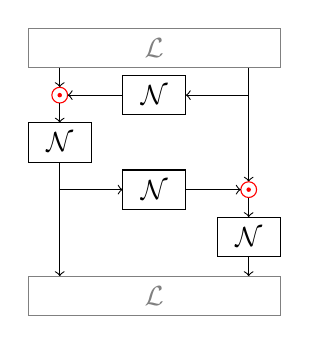
\begin{tikzpicture}[xscale=0.8,yscale=-0.5]
            \draw[color=gray] (-0.5,0.0) rectangle (3.5,1.0) node[pos=0.5] {$\mathcal{L}$};
            \draw[->] (0.0,1.0) -- (0.0,1.5);
            \draw[color=red] (0.0,1.7) ellipse (0.125 and 0.2);
            \fill[red] (0.0,1.7) ellipse (0.0357142857143 and 0.0571428571429);
            \draw (3.0,1.0) -- (3.0,1.7);
            \draw[->] (3.0,1.7) -- (2.0,1.7);
            \draw (1.0,1.2) rectangle (2.0,2.2) node[pos=0.5] {$\mathcal{N}$};
            \draw[->] (1.0,1.7) -- (0.125,1.7);
            \draw[->] (0.0,1.9) -- (0.0,2.4);
            \draw (-0.5,2.4) rectangle (0.5,3.4) node[pos=0.5] {$\mathcal{N}$};
            \draw (0.0,3.4) -- (0.0,4.1);
            \draw[->] (3.0,1.7) -- (3.0,3.9);
            \draw[color=red] (3.0,4.1) ellipse (0.125 and 0.2);
            \fill[red] (3.0,4.1) ellipse (0.0357142857143 and 0.0571428571429);
            \draw[->] (0.0,4.1) -- (1.0,4.1);
            \draw (1.0,3.6) rectangle (2.0,4.6) node[pos=0.5] {$\mathcal{N}$};
            \draw[->] (2.0,4.1) -- (2.875,4.1);
            \draw[->] (3.0,4.3) -- (3.0,4.8);
            \draw (2.5,4.8) rectangle (3.5,5.8) node[pos=0.5] {$\mathcal{N}$};
            \draw[->] (0.0,4.1) -- (0.0,6.3);
            \draw[->] (3.0,5.8) -- (3.0,6.3);
            \draw[color=gray] (-0.5,6.3) rectangle (3.5,7.3) node[pos=0.5] {$\mathcal{L}$};
        \end{tikzpicture}
    \end{subfigure}
    \centering
    \begin{subfigure}{0.45\textwidth}
        \centering
        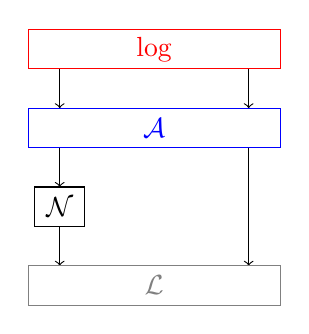
\begin{tikzpicture}[xscale=0.8,yscale=-0.5]
            \draw[color=red] (-0.5,0.0) rectangle (3.5,1.0) node[pos=0.5] {$\log$};
            \draw[->] (0.0,1.0) -- (0.0,2.0);
            \draw[->] (3.0,1.0) -- (3.0,2.0);
            \draw[color=blue] (-0.5,2.0) rectangle (3.5,3.0) node[pos=0.5] {$\mathcal{A}$};
            \draw[->] (0.0,3.0) -- (0.0,4.0);
            \draw (-0.4,4.0) rectangle (0.4,5.0) node[pos=0.5] {$\mathcal{N}$};
            \draw[->] (0.0,5.0) -- (0.0,6.0);
            \draw[->] (3.0,3.0) -- (3.0,6.0);
            \draw[color=gray] (-0.5,6.0) rectangle (3.5,7.0) node[pos=0.5] {$\mathcal{L}$};
        \end{tikzpicture}
    \end{subfigure}
    \FigDef{simplified}{A simplified view of two decompositions of $\pi$.
        Linear (resp. nonlinear) functions are denoted $\mathcal{L}$ (resp. $\mathcal{N}$ ).
        $\fmult$ denotes finite field multiplication and $\mathit{log}$ is a finite field logarithm.
        $\mathcal{A}$ denotes a simple integer arithmetic layer.
        %Linear functions are represented in grey, finite field operations in red and integer operations in blue.
        }
\end{figure}
